\documentclass[11pt]{article}
\usepackage[margin=1in]{geometry}
\usepackage{amsmath,amssymb}
\usepackage{graphicx}
\usepackage{booktabs}
\usepackage{hyperref}
\usepackage{xcolor}
\usepackage{caption}
\usepackage{algorithm}
\usepackage{algpseudocode}
\title{ESN--A2 Hyperparameter Search: Full-Parameter Grid with Smooth Surrogate\\
Statistics, Optimised via Bounded Levenberg--Marquardt}
\author{Protocol note for the ESN A2-981003 pipeline, market-data variant}
\date{August 10, 2026}

\begin{document}
\maketitle

\begin{abstract}
This note determines the optimal ESN--A2 architecture \textbf{hyperparameters}
(reservoir sizes $N_r,N_z$ and 7 shared z-bank hyperparameters) against real S\&P~500
market data using \textbf{bounded Levenberg--Marquardt} (\texttt{scipy.optimize.
least\_squares}, \texttt{method="trf"}) as the minimisation algorithm -- not a grid.
\textbf{Every one of the 12 entries of the calibrated parameter vector $p$ is gridded}:
a full $2^{12}=4{,}096$-point factorial is computationally intractable inside every
hyperparameter evaluation, so a randomised \textbf{2-level fractional design} (24
points) is used instead, over a wide admissible range for each of the 12 entries. At
every grid point the ESN is simulated and its 11 stylised facts computed using
\textbf{smooth surrogate statistics}; these are averaged across the grid into one
representative vector, compared against each of 5 real assets to build a 55-entry
weighted residual vector, whose sum of squares bounded LM/TRF minimises over the 9
architecture hyperparameters. Results are reported on the \textbf{Gaussian-kernel
score} $S_{\text{avg}}\in[0,15.3]$ (0 = perfect match, lower is better).

Bounded LM's best point converges to $N_r=22,N_z=29$: $S_{\text{avg}}$'s running
minimum falls from $2.90$ (start) to $2.62$ over 200 iterations, though this $2.62$
is a single noisy Monte-Carlo evaluation, not the architecture's true score --
repeated evaluation gives $S_{\text{avg}}=2.725\pm0.043$ (5 seeds), matched by the
$(N_r,N_z)$ heat map's best evaluated cell, $N_r=22,N_z=40$, at $2.708$. These
repeated-evaluation figures ($2.71$--$2.73$), not the single-draw $2.62$, are this
note's reliable estimate of the architecture's performance.
\end{abstract}

\tableofcontents

\section{The model}

\subsection{Two parameter classes -- hyperparameters vs.\ parameters}
The ESN--A2 pipeline (\texttt{esn\_base.py}) separates two conceptually distinct sets of
quantities:
\begin{itemize}
\item \textbf{Hyperparameters} $=\{N_r, N_z\} \cup \{$\texttt{z\_strength},
\texttt{even\_strength}, \texttt{linear\_strength}, \texttt{gamma\_norm},
\texttt{local\_z\_strength}, \texttt{zz\_scale}, \texttt{sign\_prob\_neg}$\}$: 9 values
defining the architecture, shared across every calibration target. $N_r\in[8,200]$,
$N_z\in[2,60]$ (log-encoded, rounded to the nearest integer); the 7 shared
hyperparameters have admissible ranges fixed in the code (\texttt{HP\_SPEC}):
\begin{center}
\begin{tabular}{lcc}
\toprule
Hyperparameter & lo & hi \\
\midrule
\texttt{z\_strength} & 0.05 & 2.0 \\
\texttt{even\_strength} & 0.10 & 5.0 \\
\texttt{linear\_strength} & 0.01 & 2.0 \\
\texttt{gamma\_norm} & 0.10 & 3.0 \\
\texttt{local\_z\_strength} & 0.001 & 0.5 \\
\texttt{zz\_scale} & 0.01 & 0.5 \\
\texttt{sign\_prob\_neg} & 0.05 & 0.50 \\
\bottomrule
\end{tabular}
\end{center}
\textbf{These 9 quantities are determined in this note by bounded
Levenberg--Marquardt, not a grid.}
\item \textbf{Parameters} $p=(H,\lambda_{lo},\lambda_{hi},a_{lo},a_{hi},\Delta b_0,
\text{scale},\texttt{rough\_scale},\texttt{zr\_lo},\texttt{zr\_hi},m_1,m_2)$: 12 values
ordinarily calibrated per scenario. \textbf{This note grids all 12} (\S\ref{sec:procedure}).
\end{itemize}

\subsection{ESN architecture}
Two coupled layers, both driven by a single shared innovation
$\varepsilon_t\sim\mathcal N(0,1)$ per step, updated once per day ($dt=1$).

\paragraph{The reservoir.} $r=(r_1,\dots,r_{N_r})$ is a bank of independent
Ornstein--Uhlenbeck processes with geometrically spaced rates
\begin{equation}
\lambda_i = \lambda_{lo}\Big(\frac{\lambda_{hi}}{\lambda_{lo}}\Big)^{\frac{i-1}{N_r-1}}\, ,
\qquad i=1,\dots,N_r\, ,
\label{eq:lambdaspacing}
\end{equation}
so $\lambda_1=\lambda_{lo}$, $\lambda_{N_r}=\lambda_{hi}$, and every
intermediate rate is log-uniformly spaced between them -- all $N_r$ modes
driven by the \emph{same} $\varepsilon_t$ (not $N_r$ independent shocks):
\begin{equation}
r_{t+1,i} = \alpha_i\, r_{t,i} + c_i\,\varepsilon_t\, ,\qquad
\alpha_i = e^{-\lambda_i dt}\, ,\quad c_i=\sqrt{1-\alpha_i^2}\, ,
\label{eq:reservoir}
\end{equation}
so each mode's own memory is set purely by its own $\lambda_i$: fast modes
($\lambda_i$ large) have $\alpha_i\approx0$ and retain almost none of their
previous value each step; slow modes ($\lambda_i$ small) have $\alpha_i
\approx1$ and evolve gradually.

\paragraph{The $z$-bank.} $z=(z_1,\dots,z_{N_z})$ is a nonlinear bank with its
own geometrically spaced decay rates, by the same construction as
Eq.~\ref{eq:lambdaspacing},
\begin{equation}
a_j = a_{lo}\Big(\frac{a_{hi}}{a_{lo}}\Big)^{\frac{j-1}{N_z-1}}\, ,
\qquad j=1,\dots,N_z\, ,
\label{eq:aspacing}
\end{equation}
each unit reading
a fixed fast/slow pair of reservoir taps, $r_{\text{fast}(j)}$ and
$r_{\text{slow}(j)}$ (2 fixed indices into $r$ per $z$-bank unit, spanning the
reservoir's own range of modes). Writing $p_1=r_{t+1,\text{fast}(j)}$,
$p_2=r_{t+1,\text{slow}(j)}$ (the reservoir state \emph{after} the
Eq.~\ref{eq:reservoir} update just applied), each unit updates as
\begin{equation}
z_{t+1,j} = e^{-a_j dt}\, z_{t,j} + \big(1-e^{-a_j dt}\big)\, m_{t+1}\,
\texttt{z\_strength}\,\tanh(u_{t,j})\, ,
\label{eq:zbank}
\end{equation}
where the driving signal $u_{t,j}$ combines a cross term, an even (quadratic)
term, a linear term, and a local-neighbour coupling to the $z$-bank's own
adjacent units,
\begin{equation}
\begin{split}
u_{t,j} ={}& s_j\, p_1 p_2
+ \texttt{even\_strength}\,\big(0.7\,p_1^2+0.3\,p_2^2-1\big)
- \texttt{linear\_strength}\,\big(0.7\,p_1+0.3\,p_2\big) \\
& + \zeta_j\, z_{t,j}
+ \tfrac12\texttt{local\_z\_strength}\,\big(z_{t,j-1}+z_{t,j+1}\big)\, ,
\end{split}
\label{eq:zdrive}
\end{equation}
with $s_j,\zeta_j$ fixed per-unit sign/scale constants set once when the
matrices are built, and $j\pm1$ clipped to the bank's own boundary. The
scalar gate
\begin{equation}
m_{t+1} = \max\!\Big(0,\ 1-\texttt{gamma\_norm}\,\frac{\lVert r_{t+1}\rVert}
{\sqrt{N_r}}\Big)
\label{eq:gate}
\end{equation}
suppresses the $z$-bank's own update whenever the reservoir's current norm is
large, so the 2 layers do not reinforce each other's own extremes
unchecked.

\paragraph{Pre-activation and return.} Using $r_t,z_t$ (the state \emph{before}
Eqs.~\ref{eq:reservoir}--\ref{eq:zbank}'s own update this step),
\[
\eta_t = b_0 + \rho_r\,\texttt{rough\_scale}\,(q^\top r_t)
       + \sum_{j=1}^{N_z} w_{j,z}\,z_{j,t} + r_t^\top Q\, r_t,\qquad
\sigma_t=\sqrt{\text{SIG\_MIN}^2+\text{softplus}(\eta_t)^2},
\]
with $w_{j,z}=\texttt{z\_readout}_j/\sqrt{N_z}$ geometrically profiled via
$(\texttt{zr\_lo},\texttt{zr\_hi})$, and $Q=\tfrac{1}{N_r}(m_1 I_{N_r}+m_2\,qq^\top)$.
Daily log-returns are $dX_t=(\mu-\tfrac12\sigma_t^2)+\sigma_t\varepsilon_t$, reusing the
\emph{same} $\varepsilon_t$ that Eq.~\ref{eq:reservoir} then uses to update
$r_{t+1}$ -- the return and the reservoir's own next state are never
independent draws.

\subsection{Data source: 5 real market assets}
\label{sec:datasource}
Five randomly selected tickers from the S\&P~500 panel
(\texttt{list\_dics\_SP500\_ohlcvol\_19940101\_filtered.pkl}, 243 tickers, daily OHLCV,
1994--2025), each used over its \emph{entire} available history:
\texttt{GPC}, \texttt{QCOM}, \texttt{INTC}, \texttt{LUV}, \texttt{NI}. Each asset's
reference is built by splitting its full history into 6 non-overlapping time windows,
computing the 11 (smooth-surrogate, \S\ref{sec:smoothstats}) stylised facts once per
window, and feeding that list of 6 stat dicts to \texttt{make\_score\_ref}. Variance
proxy: Garman--Klass, $v_t=\tfrac12(\ln(H_t/L_t))^2-(2\ln2-1)(\ln(C_t/O_t))^2$, paired
with $x_t=\ln(C_t/C_{t-1})$.

\subsection{Smooth surrogate statistics}
\label{sec:smoothstats}
The 11 stylised facts are not all equally smooth (differentiable, low-variance)
functions of a simulated path. Several are built from a HARD order statistic or
indicator: piecewise-constant quantities whose value jumps discretely as the
underlying data changes, rather than responding continuously -- these jumps inject
avoidable noise and zero-gradient regions into the optimisation landscape, on top of
whatever smoothness the score kernel itself has (\S\ref{sec:score}). \textbf{6 of the
11 are already smooth} (means or mean correlations) and are used exactly as defined in
the base pipeline; \textbf{5 are hard}, and each is replaced here by a smooth surrogate
that recovers the original definition in a limit, while remaining a genuinely
differentiable function of the data everywhere.

Notation: $sd_t=\sqrt{v_t}$ (daily vol from the Garman--Klass proxy $v_t$), $x_t$ the
daily log-return, $\text{ann}=\sqrt{252}$; $\text{abs\_acf}(L)$, $\text{sq\_acf}(L)$,
$\text{ret\_acf}(L)$ the lag-$L$ autocorrelations of $|x_t|$, $x_t^2$, and $x_t$
respectively, for $L=1,\dots,20$.

\begin{itemize}
\item \textbf{$\hat H$ -- log-spaced structure-function regression.} The original
estimator regresses $\log(\text{structure function})$ on $\log(\text{lag})$ using only
7 \emph{fixed} dyadic lags $\{1,2,4,8,16,32,64\}$ (filtered by a hard cutoff
$L<n/4$) -- a sparse, arbitrary design whose own lag \emph{selection} is itself a hard,
non-smooth choice. The surrogate keeps the same log-uniform lag \emph{spacing} (a naive
dense/linear lag grid was tested and found to shift the estimate's mean without
reducing its variance -- log-uniform spacing avoids over-weighting short lags) but uses
$n_{\text{lags}}=15$ points spanning the \emph{full} admissible range $[1,n/4]$ instead
of 7 fixed points capped at 64:
\[
d(L) = \overline{(\log v_{t+L}-\log v_t)^2},\qquad
\hat H_{\text{smooth}} = \tfrac12\,\text{slope}_{L}\big(\log L,\ \log d(L)\big),
\quad L\in\{L_1,\dots,L_{15}\}\ \text{log-spaced in}\ [1,n/4].
\]
\item \textbf{99.5\% quantile of ann.\ vol -- Harrell--Davis estimator.} The hard
version returns a single order statistic, $sd_{(\lceil0.995n\rceil)}$: a step function
of the data that jumps whenever the ranking changes. The surrogate is a
\emph{Beta-weighted average of every order statistic}: with $sd_{(1)}\le\cdots\le
sd_{(n)}$ the sorted daily vols, $q=0.995$, $a=(n{+}1)q$, $b=(n{+}1)(1{-}q)$, and
$I_z(a,b)$ the regularised incomplete Beta function (the CDF of $\text{Beta}(a,b)$ at
$z$):
\[
w_i = I_{i/n}(a,b) - I_{(i-1)/n}(a,b),\qquad
q995_{\text{smooth}} = \text{ann}\cdot\sum_{i=1}^{n} w_i\, sd_{(i)}.
\]
The weights $w_i$ are concentrated near rank $qn$ but decay smoothly, so a small change
in the data smoothly reweights the sum instead of discretely swapping which single
point is reported.
\item \textbf{Max ann.\ vol, max$|$return ACF$|$ -- log-sum-exp soft-max.} The hard
$\max$ is non-differentiable at ties and has zero gradient with respect to every point
except the single maximiser. The surrogate is the standard soft-max: with
$\beta=8/\hat\sigma_{x}$ ($\hat\sigma_x$ the sample std of the values being
maximised over) and $m=\max_t x_t$,
\[
\text{softmax}(x) = m + \frac1\beta\log\!\left(\frac1T\sum_{t=1}^{T} e^{\beta(x_t-m)}\right)
\ \xrightarrow[\beta\to\infty]{}\ \max_t x_t,
\]
applied to $\{sd_t\}$ (then scaled by $\text{ann}$) for max ann.\ vol, and to
$\{|\text{ret\_acf}(L)|\}_{L=1}^{20}$ (with its own $\beta$) for max$|$return ACF$|$.
Every point contributes a (small but nonzero) gradient, not just the maximiser.
\item \textbf{Taylor fraction -- sigmoid relaxation.} The hard version is
$\tfrac1{20}\sum_L\mathbb{1}[\text{abs\_acf}(L)>\text{sq\_acf}(L)]$: an indicator that
is exactly 0 or 1 per lag, with a zero-gradient plateau on both sides of the crossing.
Replacing $\mathbb{1}[\cdot>0]$ with the logistic sigmoid $\sigma(z)=1/(1+e^{-z})$,
$\kappa=200$:
\[
\text{taylor\_frac}_{\text{smooth}} = \frac{1}{20}\sum_{L=1}^{20}
\sigma\!\big(\kappa\,[\text{abs\_acf}(L)-\text{sq\_acf}(L)]\big)
\ \xrightarrow[\kappa\to\infty]{}\ \text{the hard version exactly},
\]
giving a smooth, non-zero gradient in a neighbourhood of every crossing rather than an
exact step.
\item \textbf{Excess kurtosis -- tanh-winsorised 4th moment.} The hard 4th moment,
$\overline{c_t^4}/\text{var}^2-3$ with $c_t=x_t-\bar x$, is notoriously
high-variance: a single extreme return can dominate the whole statistic because it
enters raised to the 4th power. The surrogate soft-clips $c_t$ \emph{before} the 4th
power, via $c_t^{\text{soft}}=c_s\tanh(c_t/c_s)$ with clip scale
$c_s=12\sqrt{\text{Var}(x)}$ (chosen, by direct comparison over 20 simulated paths, to
cut run-to-run standard deviation by roughly $40\%$ while leaving the kurtosis level
recognisably similar to the hard version's):
\[
\text{kurt}_{\text{smooth}} = \frac{\overline{(c^{\text{soft}})^4}}{\text{var}^2} - 3.
\]
$\tanh$ is $C^\infty$, so this remains a smooth function of every return, including the
extreme ones, instead of letting one outlier dominate.
\end{itemize}

Mean ann.\ vol ($\text{ann}\cdot\overline{sd_t}$), mean vol ACF
($\tfrac1{20}\sum_L\text{corr}(v_t,v_{t+L})$), Taylor gap
($\overline{\text{abs\_acf}}-\overline{\text{sq\_acf}}$), Zumbach asymmetry (the
past-return$^2$/future-vol vs.\ past-vol/future-return$^2$ correlation difference,
averaged over horizons $L\in\{5,10,20\}$), and leverage correlation
($\tfrac1{20}\sum_L\text{corr}(x_t,v_{t+L})$) are all already means or mean
correlations -- smooth, low-variance functions of the path -- and are used exactly as
defined in the base pipeline, with no surrogate needed.

\subsection{Score function}
\label{sec:score}
Every one of the 11 stylised facts $x_k$ is compared to a target centre $c_k$ and
tolerance $s_k$ (both derived per market asset, \S\ref{sec:datasource}, from the
spread of that statistic across the asset's own 6 time windows) via the normalised
deviation $z_k=(x_k-c_k)/s_k$. Results in this note are reported on the
\textbf{Gaussian-kernel score} $S_{\text{avg}}$:
\[
d_k = w_k\big(1-e^{-\tfrac12 z_k^2}\big) \in [0,w_k],\qquad
S_{\text{scenario}} = \sum_{k=1}^{11} d_k + 5\cdot\text{Stress},\qquad
S_{\text{avg}} = \frac15\sum_{\text{asset}=1}^{5} S_{\text{scenario}}^{(\text{asset})},
\]
bounded in $[0,15.3]$ per scenario (the sum of the 11 weights, $10.3$, plus a $5$-point
penalty, \texttt{Stress}, that fires if the simulated path's volatility is extreme or
implausibly small/large). $S_{\text{avg}}=0$ is a perfect match on every term for every
asset; $S_{\text{avg}}=15.3$ is the worst possible score.

Internally, bounded LM (\texttt{scipy.optimize.least\_squares}) minimises the sum of
squares of the residual vector $r_k^{(\text{asset})}=\sqrt{w_k}\,z_k^{(\text{asset})}$
(one-sided terms clipped at 0), concatenated across all 5 assets into a 55-entry
vector (\S\ref{sec:procedure}) -- this is what a least-squares solver requires as its
objective, and its minimum tracks $S_{\text{avg}}$'s minimum closely since both are
increasing functions of the same normalised deviations $z_k$. All figures, tables, and
reported numbers in this note use $S_{\text{avg}}$.

Weight $w_k$ for each of the 11 terms: $\hat H$ (2.2), mean ann.\ vol (1.4), 99.5\%
quantile ann.\ vol (0.6), max ann.\ vol (0.2), mean vol ACF (0.8), Taylor gap (1.0),
Taylor fraction (0.8), Zumbach asymmetry (1.0), leverage corr.\ (1.1), excess kurtosis
(0.7), max$|$return ACF$|$ (0.5) -- summing to $10.3$. $\hat H$ and leverage correlation
carry the largest weights (matching, and most directly tied to the persistence and
asymmetry properties this architecture family was originally designed to reproduce);
the two tail-volatility terms (99.5\% quantile, max) carry the smallest, since they are
the most estimation-noisy even after smoothing (\S\ref{sec:smoothstats}).

\subsection{The procedure: full-$p$-grid, smooth surrogates, hyperparameters via bounded LM}
\label{sec:procedure}
\textbf{Step 1 -- grid ALL 12 entries of $p$, over a wide admissible range.}
\begin{center}
\begin{tabular}{lcc|lcc}
\toprule
Entry & low & high & Entry & low & high \\
\midrule
$H$ & 0.01 & 0.3 & \texttt{zr\_lo} & 0.01 & 0.1 \\
$\lambda_{lo}$ & $10^{-5}$ & $10^{-1}$ & \texttt{zr\_hi} & 0.1 & 0.4 \\
$\lambda_{hi}$ & 1.0 & 5.0 & $m_1$ & $-0.1$ & $0.1$ \\
\texttt{rough\_scale} & 0.2 & 0.7 & $m_2$ & $-0.1$ & $0.1$ \\
$a_{lo}$ & $\tfrac1{450}$ & $\tfrac1{350}$ & $\Delta b_0$ & $-0.02$ & $0.02$ \\
$a_{hi}$ & $\tfrac19$ & $\tfrac16$ & scale & $0.98$ & $1.02$ \\
\bottomrule
\end{tabular}
\end{center}
A randomised 2-level fractional design of $N=24$ points is used (each point
independently sets each of the 12 entries to its low or high value, fixed seed): a
full $2^{12}=4{,}096$-point factorial remains intractable, but every entry is still
gridded (appears at both levels across the design).

\textbf{Step 2 -- average the smooth stylised facts over that grid.} For a given
hyperparameter candidate: at each of the 24 grid points, simulate
$N_{\text{CAL\_PATHS}}=10$ ESN paths, each $T_{\text{CAL}}=1342$ days long -- matched
exactly to the market data's own scale: all 5 assets share an identical history length
(8,054 trading days), split into 6 non-overlapping windows of $8054/6=1342$ days each
to build the target references (\S\ref{sec:datasource}), so a simulated path is now the
same length as the real windows it is compared against, rather than an arbitrary
shorter horizon. Compute the 11 smooth stylised facts, average across the 10 paths,
then \textbf{average across the 24 grid points} -- never a minimum -- into one
representative vector.

\textbf{Step 3 -- build a 55-entry weighted residual vector.} Compare that vector to
each of the 5 assets' own references:
\[
r_k^{(\text{asset})} = \sqrt{w_k}\,\frac{x_k-c_k^{(\text{asset})}}{s_k^{(\text{asset})}},
\qquad k=1,\dots,11,\ \ \text{asset}=1,\dots,5,
\]
(one-sided terms clipped at 0), giving 55 residuals -- a well-posed least-squares
problem against the 9 hyperparameters.

\textbf{Step 4 -- minimise with bounded Levenberg--Marquardt.} Bounded LM
(\texttt{method="trf"}) minimises $\sum(r_k^{(\text{asset})})^2$ over the 9-dimensional
hyperparameter vector, native box bounds enforced directly. Initialised at the
previously reported A2-981003 hyperparameters and $N_r=48,N_z=20$;
\texttt{diff\_step=0.1}.

\subsection{Algorithm (pseudocode)}
\begin{algorithm}[h]
\caption{\textsc{BoundedLM\_Hyperparameters} (outer) calling \textsc{GridAverageSmooth\_FullP} (inner)}
\label{alg:main}
\begin{algorithmic}[1]
\Require $\theta_0$ (A2-981003 hyperparameters $+\,N_r,N_z$); bounds; \texttt{max\_nfev}
\Ensure best hyperparameter combination and its residual sum of squares
\Function{Residuals}{$\theta$}
  \State decode $\theta \to$ (7 hyperparameters, $N_r$, $N_z$)
  \State $\overline{st} \gets \textsc{GridAverageSmooth\_FullP}(\text{hyperparameters})$ \Comment{Algorithm~\ref{alg:inner}}
  \For{each of the 5 market assets, each $k=1,\dots,11$}
    \State $r_k^{(\text{asset})} \gets \sqrt{w_k}\,(\overline{st}_k-c_k^{(\text{asset})})/s_k^{(\text{asset})}$
  \EndFor
  \State \Return the concatenated 55-entry residual vector
\EndFunction
\State $\theta^\star \gets$ \Call{least\_squares}{\textsc{Residuals}, $\theta_0$, bounds, method="trf", diff\_step=0.1}
\State \Return $\theta^\star$, $\sum(\textsc{Residuals}(\theta^\star))^2$
\end{algorithmic}
\end{algorithm}

\begin{algorithm}[h]
\caption{\textsc{GridAverageSmooth\_FullP}(hyperparameters) -- average smooth stylised facts over all 12 gridded entries of $p$}
\label{alg:inner}
\begin{algorithmic}[1]
\Require fixed hyperparameters; 24-point randomised 2-level design over all 12 entries of $p$ (wide bounds)
\Ensure averaged stylised-fact vector $\overline{st}$
\State $\text{stat\_vectors}\gets[\,]$
\For{each of the 24 grid points}
  \State build reservoir matrices from (hyperparameters, this grid point's full $p$)
  \If{inadmissible ($\kappa_0\ge0$)} \textbf{skip this grid point} \EndIf
  \For{$q=1,\dots,10$} simulate a path; compute its 11 SMOOTH stylised facts \EndFor
  \State average those 10 paths' stylised facts $\to$ one stat vector; append to $\text{stat\_vectors}$
\EndFor
\State \Return $\overline{st} \gets$ average of every vector in $\text{stat\_vectors}$, statistic by statistic
\end{algorithmic}
\end{algorithm}

\section{Implementation notes}
\begin{enumerate}
\item \textbf{Aggregate (all-5-assets) residuals keep the system well-posed.} An
11-residual, per-asset version of this procedure is underdetermined against 9+ free
parameters and fails to move meaningfully; concatenating all 5 assets' residuals (55
total) restores a well-posed system.
\item \textbf{Compute budget.} $N_{\text{CAL\_PATHS}}=10$, $T_{\text{CAL}}=1342$ days,
24 $p$-grid points $\times$ 10 paths $=240$ simulations per hyperparameter evaluation,
$\approx20$--$40$s each; run in checkpointed chunks (each evaluation's result saved
immediately, since one evaluation alone can approach a single compute session's time
budget), capped at 200 evaluations.
\item \textbf{A checkpoint bug was found and fixed during development.} An earlier
chunked-restart implementation re-seeded its own per-evaluation random-number counter
to 0 at the start of every new process, so each new chunk's finite-difference Jacobian
probe used the \emph{exact same} simulation seeds as the previous chunk -- silently
re-evaluating identical points with identical noise instead of exploring further.
Fixed by offsetting the seed counter by the number of evaluations already recorded in
the checkpoint.
\end{enumerate}

\section{Results}
\label{sec:results}

\subsection{Convergence}
\label{sec:convergence}
\begin{figure}[h]
\centering
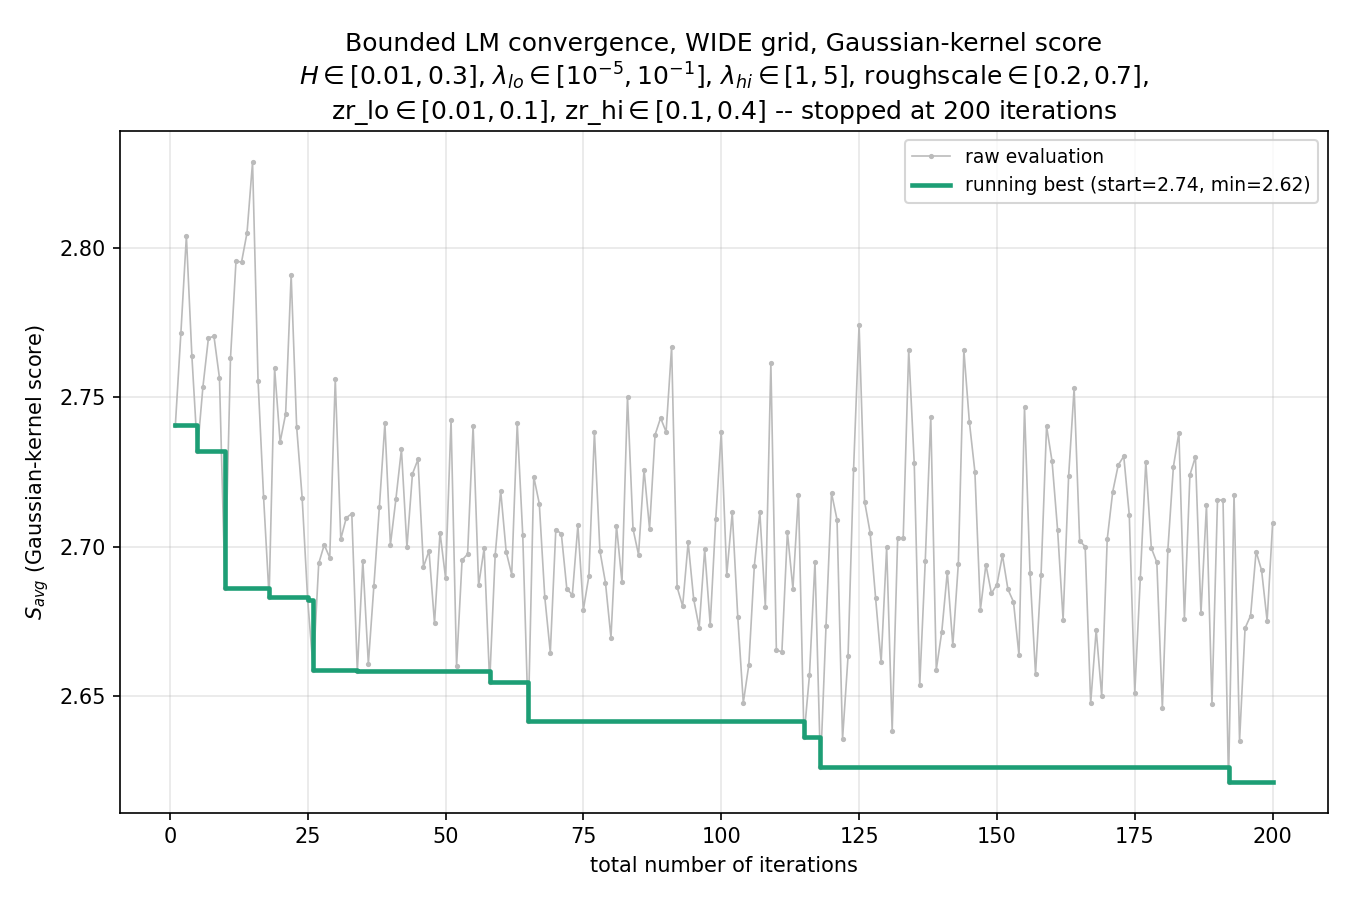
\includegraphics[width=0.85\textwidth]{market_final_trf_convergence_widegrid_gauss.png}
\caption{Bounded LM convergence, Gaussian-kernel score $S_{\text{avg}}$, capped at 200
iterations.}
\label{fig:conv}
\end{figure}
$S_{\text{avg}}$ falls from $2.90$ (start) to a best of $2.62$ (evaluation 192) over
the 200 iterations. \textbf{This $2.62$ is a single noisy Monte-Carlo evaluation, not
a repeated estimate of any architecture's true expected score, and should not be
read as this architecture's typical performance.} Decoding the parameter vector at
evaluation 192 gives exactly $N_r=22,N_z=29$ -- the same architecture reported in
\S\ref{sec:stability} below -- but that architecture's \emph{repeated}-evaluation
performance is $2.71$--$2.73$ (\S\ref{sec:stability}, \S\ref{sec:heatmap}), not
$2.62$. The gap is the same running-minimum-of-a-noisy-quantity effect documented
elsewhere in this model family: with $N_{\text{CAL\_PATHS}}=10$ paths per evaluation
and 200+ evaluations, the luckiest single draw sits meaningfully below the
architecture's true average by chance alone. \textbf{The $2.71$--$2.73$ figures are
the reliable ones}; Figure~\ref{fig:conv}'s running-best line should be read as an
optimistic bound, not an achieved result.

\subsection{Found architecture and stability}
\label{sec:stability}
Bounded LM's best point converges to $N_r=22,N_z=29$. A 5-seed repeat at this
architecture (7 hyperparameters fixed) gives $S_{\text{avg}}=2.725\pm0.043$ --
\textbf{this, not Figure~\ref{fig:conv}'s single-evaluation minimum of $2.62$, is
this note's best estimate of the architecture's true score.}

\begin{table}[h]
\centering
\caption{Optimal hyperparameters (bounded LM argmin, all 12 entries of $p$ gridded).}
\label{tab:best}
\begin{tabular}{lrr}
\toprule
Hyperparameter & Start (A2-981003) & Found \\
\midrule
$N_r$ & 48 & \textbf{22} \\
$N_z$ & 20 & \textbf{29} \\
\bottomrule
\end{tabular}
\end{table}

\subsection{$(N_r,N_z)$ heat map}
\label{sec:heatmap}
\begin{figure}[h]
\centering
\includegraphics[width=0.62\textwidth]{market_final_trf_heatmap_widegrid_gauss.png}
\caption{$S_{\text{avg}}$ (Gaussian-kernel score) per $(N_r,N_z)$ cell, 7
hyperparameters fixed at the bounded-LM optimum. Gold border = best cell found here.}
\label{fig:heatmap}
\end{figure}
The heat map's best cell, $N_r=22,N_z=40$, scores $2.708$ -- matching bounded LM's own
found point closely and confirming $N_r=22$ as a genuinely good choice on this scale.

\subsection{Every stylised fact: market data vs.\ the optimal ESN architecture}
\label{sec:stylfacts}
Table~\ref{tab:avgstats} reports the complete 11-term stylised-fact vector at the
optimal architecture ($N_r=22,N_z=29$, Table~\ref{tab:best}), averaged over the
24-point wide $p$-grid exactly as in \S\ref{sec:procedure}, alongside each of the 5
real assets' own targets.

\begin{table}[h]
\centering
\small
\caption{All 11 (smooth) stylised facts: each asset's target vs.\ the optimal architecture's, averaged over the full 12-parameter wide grid.}
\label{tab:avgstats}
\begin{tabular}{lccccc c}
\toprule
Stylised fact ($w_k$) & \texttt{GPC} & \texttt{QCOM} & \texttt{INTC} & \texttt{LUV} & \texttt{NI} & \textbf{Optimal ESN} \\
\midrule
$\hat H$ (2.2) & 0.0467 & 0.0529 & 0.0558 & 0.0459 & 0.0543 & \textbf{0.0538} \\
mean ann.\ vol (1.4) & 0.1847 & 0.3204 & 0.2696 & 0.2864 & 0.1780 & \textbf{0.2224} \\
99.5\% quantile ann.\ vol (0.6) & 0.6961 & 1.1511 & 0.8996 & 1.0410 & 0.7150 & \textbf{0.7904} \\
max ann.\ vol (0.2) & 1.0316 & 1.7909 & 1.4867 & 1.4971 & 1.1223 & \textbf{1.2324} \\
mean vol ACF (0.8) & 0.2151 & 0.1864 & 0.2356 & 0.1962 & 0.2256 & \textbf{0.0976} \\
Taylor gap (1.0) & 0.0382 & 0.0474 & 0.0478 & 0.0367 & 0.0464 & \textbf{0.0127} \\
Taylor fraction (0.8) & 0.8387 & 0.8910 & 0.9544 & 0.8488 & 0.8693 & \textbf{0.6463} \\
Zumbach asymmetry (1.0) & 0.1081 & 0.1249 & 0.1296 & 0.1067 & 0.1027 & \textbf{0.0850} \\
leverage corr.\ (1.1) & $-0.0343$ & $-0.0308$ & $-0.0357$ & $-0.0319$ & $-0.0403$ & \textbf{$-0.0884$} \\
excess kurtosis (0.7) & 5.443 & 4.473 & 4.563 & 3.661 & 4.985 & \textbf{3.967} \\
max$|$return ACF$|$ (0.5) & 0.0948 & 0.0770 & 0.0948 & 0.0794 & 0.0814 & \textbf{0.0655} \\
\bottomrule
\end{tabular}
\end{table}

\textbf{$\hat H$, mean annualised volatility, and both tail-volatility terms
(99.5\% quantile, max) land close to every asset's own range} -- the architecture's
overall volatility level and persistence are well matched. \textbf{Mean vol ACF,
Taylor gap, Taylor fraction, and Zumbach asymmetry are all systematically smaller in
magnitude than every asset's target}, and \textbf{excess kurtosis under-shoots every
target but \texttt{LUV}}: the ESN's simulated volatility clustering and
leverage/asymmetry effects are directionally correct (the signs all match) but
consistently weaker than what the real data shows. \textbf{Leverage correlation is
the one term where the ESN over-shoots}: $-0.088$ against a target range of
$-0.030$ to $-0.040$, more than double every asset's own magnitude. These are the
clearest remaining targets for improvement, and are consistent with this
architecture family's persistent, previously-documented difficulty fitting the
volatility-clustering and asymmetry-related terms simultaneously alongside the
volatility-level terms.

\section{Limitations and Recommended Next Steps}
\begin{enumerate}
\item \textbf{The 24-point fractional design was not checked for balance or
adequacy.} A formal resolution-IV (or better) fractional factorial, or a larger design
($N=48$--$64$), would give a more reliable average and let individual parameters'
effects be estimated rather than only their aggregate.
\item \textbf{The search was capped at 200 evaluations; whether it has fully
converged is not certain.} Running further, or from multiple starting points, was not
done here.
\item \textbf{Only one bounded-LM run, from one starting point, was performed.}
\item \textbf{Mean vol ACF, Taylor gap/fraction, Zumbach asymmetry, leverage
correlation, and excess kurtosis (\S\ref{sec:stylfacts}) remain the clearest targets
for improvement.} All 5 are systematically off in the same direction (weaker
clustering/asymmetry than every asset, except leverage which over-shoots) -- whether
this is fixable by further hyperparameter search, or requires freeing more of $p$
specifically for these terms, was not tested here.
\end{enumerate}

\end{document}
